%!Mode:: "TeX:UTF-8"
%!TEX program  = xelatex

%\documentclass{cumcmthesis}
\documentclass[withoutpreface,bwprint]{cumcmthesis} %去掉封面与编号页
\usepackage{tikz}

\usepackage{url}
\usepackage[numbers,sort&compress]{natbib}
\usepackage[ruled,vlined]{algorithm2e}

\title{基于链路预测对老龄化的分析}
\tihao{C}
\baominghao{202022006037}
\schoolname{西南大学}
\membera{王瑜瑶}
\memberb{宋行健}
\memberc{朱素毓}
\supervisor{}
\yearinput{2020}
\monthinput{09}
\dayinput{13}

\usepackage{tikz}
\newcommand*{\circled}[1]{\lower.7ex\hbox{\tikz\draw (0pt, 0pt)circle (.5em) node {\makebox[1em][c]{\tiny #1}};}}

\begin{document}

 \maketitle
 \begin{abstract}
中小



\keywords{信贷定价\quad  随机森林\quad   朴素贝叶斯}
\end{abstract}

%目录
\tableofcontents

\newpage
\section{问题重述}
随着贷


$m_2 \circled{\rm{V}} m_1$



\section{模型假设}

\begin{algorithm}[ht]
	\caption{分支限界算法实现旅行商问题}
	\label{alg:7}
	
	\KwIn{图的邻接矩阵: $G$
	}
	\KwOut{最优解和最优值}
	
	\BlankLine
	
	初始化最小堆;\\
	
	\While{遍历每一层 E.s<(n-1)}{
		\If{当前扩展结点是叶结点的父结点(到了n-2层)}{
			\If{形成回路且当前值优于最优值或还未产生最优值}{
					更新最优解;\\
					更新最优值;\\
			}
			\Else{舍弃需要进一步搜索的节点;}
		}
		\Else{
			\For{遍历这个节点的所有扩展节点}{
				\If{这个点可以进入下一个未访问的点}{
					更新当前费用;\\
					更新最小出边费用和;\\
					更新下界(限界函数);\\
					\If{子树可能含最优解}{
						节点插入最小堆;\\
					}
				}
			}
		完成当前节点的扩展,清除该节点;\\
	}
	\If{最小堆已经空}{结束循环}
	从最小堆中弹出队首节点 E;\\
	}
	
	\end{algorithm}

\begin{algorithm}[ht]
	\caption{回溯算法实现n皇后问题}
	\label{alg:6}
	
	\KwIn{棋盘数组: $Chess[N][N]$, 递归到第n层: $n$
	}
	\KwOut{所有放置皇后的方案和方案总数}
	
	\BlankLine
	
	\If{到了第$(n+1)$层(已经成功放置最后一个皇后)}{
		格式化出处当前解决方案;\\
		返回上一层;\\
	}
	\Else{
		\For{遍历这一层的每一个点}{
				\If{这个点满足放置皇后的条件}{
					放置皇后;\\
					进入下一层递归;\\
					移走皇后;\\
				}
			}
	}	
\end{algorithm}

\begin{algorithm}[ht]
	\caption{回溯算法实现旅行售货员问题}
	\label{alg:5}
	
	\KwIn{递归到第n层: $n$
	}
	\KwOut{最优解和最优值}
	
	\BlankLine
	
	\If{到了第$n$层(已经成功访问了所有节点)}{
		\If{形成回路(当前点和上一个点有连线,且和第$1$个点有连线)}{
			\If{当前值优于最优值或还未产生最优值}{
				更新最优解;\\
				更新最优值;\\
			}
		}
		返回上一层;\\
	}
	\Else{
		\For{遍历这一层的每一个点}{
			\If{这个点可以进入下一个未访问的点}{
				将这个点通过交换的方式存入解数组;\\
				累加最优值;\\
				进入下一层递归;\\
				将这个点通过交换的方式移出解数组;\\
				还原最优值;\\
			}
		}
	}	
\end{algorithm}


\begin{algorithm}[ht]
	\caption{贪心算法实现二元归并树问题}
	\label{alg:4}
	
	\KwIn{需要归并的文件长度向量 $arr$.
	}
	\KwOut{最小带权外部路径长度}
	
	\BlankLine
	
	
	对文件长度数据进行从小到大的排序;
	
	\While{当前 vector 中还有未进行归并的节点}{
		查找 vector 中当前最小的两个节点;\\
		将这两个节点进行归并,并打上标记(赋值为正无穷);\\
		将归并结果作为新的节点插入 vector;\\
		记录这两个归并节点和新节点的父节点和子节点信息;\\
		累加移动总量;\\
	}
	
	
\end{algorithm}



\begin{algorithm}[ht]
	\caption{动态规划实现矩阵连乘最优化问题}
	\label{alg:1}
	
	\KwIn{连乘矩阵行列值数组$p$; 连乘矩阵的个数$n$; 储存分步最优值矩阵的内存$m$; 储存分步最优解矩阵的内存$s$.
	}
	\KwOut{最优解}
	
	\BlankLine
	

	考虑连乘长度为1的情况,将对应矩阵运算次数的最优值都设置为0;

	\For{连乘长度,子问题规模(从2两个开始,到全部矩阵连乘)}{
		\For{连乘开始的位置,子问题定位}{
			\For{分成两部分的分割位置}{
				\If{这是子问题的最优值} {
					在矩阵$m$中进行记录最优值;\\
					在矩阵$s$中进行记录分割位置;\\
				}
				
			}
		}
	}
	
	返回最优值;
	
\end{algorithm}



\begin{algorithm}[ht]
	\caption{分治策略实现棋盘覆盖问题}
	\label{alg:2}
	
	\KwIn{棋盘的左上角坐标$(tr,tc)$; 特殊方块的位置 $(dr,dc)$; 棋盘大小$size$.
	}
	\KwOut{使用L型骨牌覆盖好的棋盘}
	
	\BlankLine
	
	骨牌编号$t$随递归次数增加;\\
	棋盘大小$size$随递归次数每次除以2增加;\\
	\textbf{(a. 覆盖左上角子棋盘)}\\
	\If{特殊方格在左上角子棋盘中} {
		递归覆盖非特殊方格的其余方格;\\
	}
	\Else{
		用$t$号L型骨牌覆盖右下角;\\
		递归覆盖其余方格;
		}
	
	\BlankLine
	\textbf{(b. 覆盖右上角子棋盘)}\\
	\If{特殊方格在右上角子棋盘中} {
		递归覆盖非特殊方格的其余方格;\\
	}
	\Else{
		用$t$号L型骨牌覆盖左下角;\\
		递归覆盖其余方格;
	}

	\BlankLine
	\textbf{(c. 覆盖左下角子棋盘)}\\
	\If{特殊方格在左下角子棋盘中} {
		递归覆盖非特殊方格的其余方格;\\
	}
	\Else{
		用$t$号L型骨牌覆盖右上角;\\
		递归覆盖其余方格;
	}

	\BlankLine
	\textbf{(d. 覆盖右下角子棋盘)}\\
	\If{特殊方格在右下角子棋盘中} {
		递归覆盖非特殊方格的其余方格;\\
	}
	\Else{
		用$t$号L型骨牌覆盖左上角;\\
		递归覆盖其余方格;
	}
	
\end{algorithm}




\begin{algorithm}[ht]
	\caption{分治策略递归实现斯特拉森矩阵乘法}
	\label{alg:3}
	
	\KwIn{\\pM1——矩阵1;\\
		nLeftIndex1,nTopIndex1——矩阵1左上角索引点(相对于源矩阵pMl);\\
		nTotalCol1——矩阵1实际使用的列数;\\
		pM2——矩阵2;\\
		nLeftIndex2, nTopIndex2——矩阵2左上角索引点(相对于源矩阵pM2);\\
		nTotalCol2——矩阵2实际使用的列数;\\
		nCount——方阵阶数n;\\
		pResult——存放运算结果矩阵的内存空间;
	}
	\KwOut{运算结果矩阵}
	
	\BlankLine
	
	

	\If{当前矩阵为2阶方阵} {
		直接进行矩阵乘法运算;\\
	}
	\Else{
		将两个矩阵分别拆分成4个大小相等的子矩阵:\\
		将矩阵1拆分为$\left(\begin{array}{ll}A_{11} & A_{12} \\ A_{21} & A_{22}\end{array}\right)$; 将矩阵2拆分为
		$\left(\begin{array}{ll}B_{11} & B_{12} \\ B_{21} & B_{22}\end{array}\right)$;\\
		
		\BlankLine
		\textbf{递归利用斯特拉森矩阵乘法得到7个小矩阵:}\\
		$\begin{aligned} 
		M_{1}=& A_{11}\left(B_{12}-B_{22}\right) \\ 
		M_{2}=&\left(A_{11}+A_{12}\right) B_{22} \\
		M_{3}=&\left(A_{21}+A_{22}\right) B_{11} \\
		M_{4}=& A_{22}\left(B_{21}-B_{11}\right) \\ 
		M_{5}=&\left(A_{11}+A_{22}\right)\left(B_{11}+B_{22}\right) \\
		M_{6}=&\left(A_{12}-A_{22}\right)\left(B_{21}+B_{22}\right) \\  M_{7}=&\left(A_{11}-A_{21}\right)\left(B_{11}+B_{12}\right) \\ 
		 \end{aligned}$
		
		\BlankLine
		\textbf{使用矩阵加减法计算得出结果矩阵的四部分:}\\
		$\begin{aligned}C_{11}=&M_{4}+M_{5}-M_{2}+M_{6}\\
		C_{12}=&M_{1}+M_{2}\\
		C_{21}=&M_{3}+M_{4}\\
		C_{22}=&M_{5}+M_{1}-M_{3}-M_{7} \end{aligned}$
		
		合并结果矩阵:
		$Result=\left(\begin{array}{ll}C_{11} & C_{12} \\ C_{21} & C_{22}\end{array}\right)$\\
		释放内存;\\
		
	}
	

\end{algorithm}





\begin{itemize}
\item 所有附件所给的数据真实且合理;
\item 不考虑其他主观因素(例如企业之间的商业竞争、银行之间的利益冲突)的影响;
\item 数据源中其他未列出的评价对企业的信誉评级没有影响;
\item 假设同一信用等级的企业能够申请的最大信贷额度是一定的;
\item 不考虑企业与银行的历史交易关系,例如企业在银行的往期存款、企业在银行的入股情况、与银行的合作时长以及在银行抵押优质资产占客户在金融机构抵押的优质资产比率等;
\item 假定贷款年限为一年,贷款额度为10-100万元,年利率为4\%-15\%。
\end{itemize}


\section{符号说明}
\begin{center}
	\begin{tabular}{lll}
		\hline
		符号		  &  意义 & 备注\\ \hline
		$W$	    & 银行的放贷盈利 & \\ \hline
		$Q_i$	    & $i$类企业的贷款额度 & 10-100万元\\ \hline
		$n_i$		&$i$类企业的个数&\\ \hline
		$r_0$		&央行出台的贷款基准利率&\\ \hline
		$r_i$	    & 银行针对$i$类企业的贷款年利率& 4\%-15\% \\ \hline
		$p_i$		&$i$类企业的风险溢价率 &\\ \hline
		$l_i$		& 客户流失率 &\\ \hline

		
	
	\end{tabular}
\end{center}



\section{问题一——LPR 定价机制下中小商业银行信贷定价模型}
\subsection{问题一的分析}
对附件1中123家企业的信贷风险进行量化分析,计算出“进项发票作废比”、“销项发票作废比”、“2016至2020年年支出”、“2016至2020年年收入”、“2016至2020年年利润”、“进项负数发票数量”、“销项负数发票数量”等初级指标,对所给数据先进行升维处理。给出该银行在年度信贷总额固定时对这些企业的信贷策略。

问题一要求对已给的123企业的信贷风险进行量化分析,并在附件一中给出了这123家企业的企业类别、信誉评级、是否违约和进出项发票的信息。

针对信贷风险的量化问题:首先,我们需要对数据进行处理,根据经济学的知识和经验计算出衡量一个企业财务和信用状况的几个指标;接着在第二问中我们利用随机森林方法对各个指标和信用水平的关系式进行确定。

针对银行的信贷策略问题 \cite{杨伟歧2011商业银行中小企业信贷策略研究}:策略由是否放贷、放贷额度、利率和期限组成。其中,放贷期限为1年;根据信用水平的量化表达式,我们通过分析企业信用水平对银行信贷利率的影响计算出不同信用等级企业的放贷利率,最后在“银行净利润最大”的优化目标下求解不同等级企业的放贷额度。

\subsection{数据预处理}
题目为我们提供了三个附件,附件中的数据给出了各企业的相关信息:附件1是123家有信贷记录企业的进销项发票信息;附件2是302家无信贷记录企业的进销项发票信息;附件3是银行贷款年利率与不同信誉评级的客户流失率的关系。
对于众多的发票信息,我们需要对数据进行清洗整理,使用EXCEL和MATLAB软件对数据做了以下预处理:
\begin{enumerate}
	\item 统计出每个公司进项、销项发票总数、发票作废数,进而计算出进销项发票作废比。
	\item 根据开票日期和进、销项发票的税价合计,统计出2016-2020年每个公司的收入、支出,进而计算出当年的利润。
	\item 我们根据《国民经济行业分类》\cite{guominjingji}对附件1中的123家企业进行了人工分类。共分为12类:餐饮业、城市建设、电器、服务业、工业、建筑与装饰、交通运输、科技密集型产业、零售业、农业、医疗、个体企业。
	\item 对数据进行归一转换,并把字符串类型特征“是”、“否”分别用“1”、“0”表示。
\end{enumerate}

\begin{figure}[h]	
	\centering
	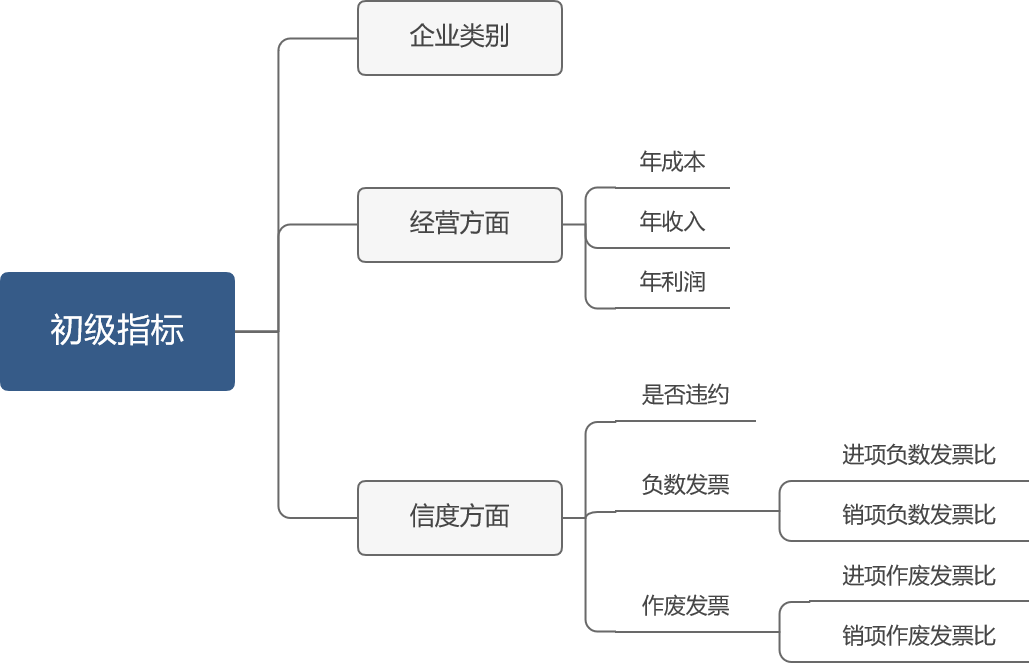
\includegraphics[width=0.7\linewidth]{fig/primary}
	\caption{初级指标}
	\label{fig:primary}
\end{figure}


\subsection{银行贷款年利率与客户流失率}\label{sec:this}
附件3中给出了银行贷款年利率与客户流失率的数值关系。其中客户流失率(Cstomer Churn Rate, CCR) \cite{Huang2018Application,张卫2018关于顾客流失率的研究} 不仅与银行设定的贷款年利率有关,也与客户企业的信誉评级有关。对于信誉评级高的企业,其可以供选取的信贷公司较多,因此会在信贷公司之间给出的年利率进行横向比较。然而,对于信誉评级较低的企业,其可供选择的信贷公司较少。

图(\ref{fig:churn})中展示的是针对A、B、C三级企业,银行贷款的不同年利率对客户流失率的关系。在下方的三个子图中,我们对关系曲线进行了多项式拟合(5阶)。得到不同信誉等级的企业流失率与利率的关系为:
\begin{equation}
\begin{array}{rcl}
l_1&=&141970x^5-72481x^4+14857x^3-1588.2x^2+96.825x-2.1004\\
l_2&=&117499x^5 - 61734x^4 + 1298x^3 - 1414.9x^2 + 87.735x - 1.9255\\
l_3&=&114626x^5 - 56609x^4 + 11257x^3 - 1183.1x^2 + 74.171x - 1.6557
\end{array}
\end{equation}

其拟合优度$R^2$均大于0.998,拟合效果良好 \cite{程维虎2000拟合优度检验的回归分析方法及其应用}。

\begin{figure}[h]	
	\centering
	\includegraphics[width=\linewidth]{fig/churn.eps}
	\caption{银行贷款年利率与客户流失率关系}
	\label{fig:churn}
\end{figure}

\subsection{基于随机森林的信贷风险量化模型}

\subsection{信贷策略的确定}
信贷策略由是否放贷、贷款额度、贷款利率和期限组成。题中所给的贷款期限为1年。根据上文得出的对某一特定企业信贷风险的量化模型,我们认为信用等级为D级的企业应不予授予放贷资格。

银行放贷的目的是为了在帮扶中小型企业的同时、实现贷款盈利最大化,由此我们可以得出数学模型:
\begin{equation}
max\;W=\sum_{i=1}^3 Q_in_ir_i(1-l_i(r_i))
$$
$$
s.t
\begin{array}{l}
10\leq Q_i\leq100\qquad i=1,2,3\\
Q_1\leq Q_2\leq Q_3= \frac{S-Q_in_1-Q_2n_2}{n_3}
\end{array}
\end{equation}

其中,$W$为银行盈利;$Q_i$为信用等级$i$的企业所得贷款额度;$r_i$为$i$类企业的贷款利率;$n_i$
为$i$类企业的数量;$l_i$为$i$类企业在贷款利率为$r_i$情况下的流失率,为\ref{sec:this}中拟合出的关系式。

接下来,我们通过建立模型对不同信用等级企业的贷款利率$r_i$、贷款额度$Q_i$进行确定。
\subsubsection{贷款利率的确定}

银行信贷业务的定价主要基于风险量化和会计核算两个角度,目前业界主要采用的定价模式有风险加点模式、成本加成模式和客户关系模式。\cite{马春明2014基于财务报表视角的邮政储蓄银行哈尔滨分行信贷风险管理研究}

其中风险加点模式是从风险溢价的角度进行定价,核心思想是:利率由基准利率和信用风险溢价组成。其代表是LPR (Loan Prime Rate) \cite{鲍毅莺2020贷款基础利率} 定价机制。

成本加成模式是从会计核算的角度对贷款进行定价,主要代表是以RAROC(Risk Adjusted Return on Capital)模型 \cite{李海涛2004RAROC} 为核心的定价机制,其核心思想是:商业银行为了创造利润,其业务成本(包括资金成本、运营成本、资本成本等)与企业违约产生的风险成本应不超过信贷产品价格。该种利润针对的主要对象是资金流较大导致银行业务成本远大于风险成本的的大型企业,不适用于本题中所给的中小型企业。

客户关系模式即为银行在计算客户信贷额度时,要将该客户有关的所有收益与费用全部纳入考虑范围,包括客户在行存款、存款资金投资收益等,是基于客户与银行的历史交易合作信息的考量,故不适用于本题。

综上,我们采用风险加点模式中的LPR信贷利率计算机制对贷款利率进行计算。LPR信贷利率计算模型如下:

\begin{equation}
r_i=r_0+bp_i
\end{equation}

其中,$r_i$为信用等级为$i$类企业的信贷利率;$r_0$为基准利率,由央行在当年颁布,经过查询,我们得到2020年的$r_0$值为$3.85\%$;$b$风险最高客户的贷款利率与$r_0$之差;$p_i$为$i$类企业的风险溢价率。

接下来我们对风险溢价率进行建模计算。

我们认为企业的风险溢价率可以由其失信率近似。企业失信率越高,则其风险溢价率越高,银行提供给企业的贷款利率就越高。因此,我们利用手上的企业票据信息和上下游企业信息对企业的失信率进行度量。

现实中不同银行的风险偏好不同。对于风险厌恶型的银行会要求更高的风险溢价,风险喜好型则相对较低。由于该模型的对象是中小微企业,其受到国家政策的扶持,且融资周期相对大型企业较短,故在模型中我们假定银行为风险中性型。根据冯·诺依曼-摩根斯坦效用函数,风险喜好型银行的效用函数为凸函数。故我们定义$i$类企业的失信率$p_i$:

\begin{equation}
p_i=\frac{1}{1+e^{-\overrightarrow{x}  \overrightarrow{\beta}}}
\end{equation}

其中$\vec x=(x_1,x_2,x_3)$,为衡量失信率的三个指标构成的三维向量,$\overrightarrow{\beta}=(\beta_1,\beta_2,\beta_3)$为三个指标的权重向量。 

下面我们定义$\vec x$。

由于样本数$n_i\;i=1,2,3$过少,不满足弱大数率的条件,故无法直接用样本失信率代替某信誉等级企业的总体失信率。因此对信用评级为$i$的企业,我们提出三个指标来衡量其失信率以增强其失信率的准确程度,分别为样本失信率$x_{i1}$、进项作废比$x_{i2}$、销项作废比$x_{i3}$。其计算公式如下:

\begin{equation}
\begin{array}{rcl}
x_{i1}&=&\frac{n_{i1}}{n_1}\\
x_{i2}&=&\frac{n_{i2}^*}{n_{i2}}\\
x_{i3}&=&\frac{n_{i3}^*}{n_{i3}}\\
\end{array}
\end{equation}

其中$n_{i1}$表示失信$i$类企业数,$n^*_{i_2}$表示$i$类企业的作废进项发票数,$n_{i_2}$表示$i$类企业的总进项发票数,$n^*_{i_3}$表示$i$类企业的作废销项发票数,$n_{i_3}$表示$i$类企业的总销项发票数。

在得到衡量失信率的三个指标之后,我们利用熵权法确定三个指标的权重。

由于三个指标的实际意义都为某种比例,且都是介于$[0,1]$之间的数,具有相同的量纲;且样本失信率和两类发票的作废率和企业失信率正相关,即都为同质正项指标,故我们不对指标进行归一化处理。

计算第$j$项指标下第$i$个样本值占该指标的比重$q_{ij}$为:

\begin{equation}
q_{ij}=\frac{x_{ij}}{\sum_{i=1}^{3}x_{ij}}\qquad i=1,2,3 \quad j=1,2,3
\end{equation}

计算第$j$项指标的信息熵冗余度$d_j$:
\begin{equation}
d_j=1+\frac{1}{3}\sum_{i=1}^{3}q_{ij}\ln q_{ij} \qquad j=1,2,3
\end{equation}

得出各项指标权重$\beta_j$:
\begin{equation}
\beta_j=\frac{d_j}{\sum_{j=1}^{3}d_j}\qquad j=1,2,3
\end{equation}

经过计算,得到三个指标的权重如下表所示:

因此最终得到的风险溢价率模型为:

\begin{equation}
p_i=\frac{1}{1+e^{-(\sum_{j=1}^3\beta_j\frac{n^*_{ij}}{n_{ij}})}} \qquad i=1,2,3
\end{equation}

综上,对于信用等级为$i$类的企业,银行提出的贷款利率$r_i$为:
\begin{equation}
r_i=r_0+\frac{b}{1+e^{-(\sum_{j=1}^3\beta_j\frac{n^*_{ij}}{n_{ij}})}} \qquad i=1,2,3
\end{equation}

其中$i=1,2,3$分别代表A,B,C三类企业,$r_0$、$b$由当年央行及商业银行颁布决定,$\beta_i$为上述表格中的值。


\subsubsection{贷款额度的确定}

通过遍历空间中的点求取银行利润$W$的最大值,我们可以得到不同信用等级企业的贷款额度的最优解,如表(\ref{tb:res})所示。

\begin{table}[h]
	\caption{信贷定价模型}
	\label{tb:res}
	\centering
	\begin{tabular}{lll}
		\hline
		信誉评级 &  贷款额度(万元)  &  年利率 \\
		\hline
		A & 100 & 4\%  \\
		B & 67 & 7\%  \\
		C & 10 & 14\%  \\
		D & 0 & -  \\
		\hline
	\end{tabular}
\end{table}

\begin{center}
	\textcircled{V}
\end{center}


%%%%%%%%%%%%%%%%%%%%%%%%%%%%%%%%%%%%%%%%%%%%%%%%%%%%%%%%%%%%%%%%%%%%%%%%%%%
\section{问题二——基于随机森林的信誉等级评定}
\subsection{问题二的分析}
在问题一的模型基础上,对待不同信誉评级的企业,我们已经具有适合的信贷方案,在问题二中我们需要应用问题一的分级信贷策略。因此,如何利用附件2中的数据对302家企业进行信誉评级成为了问题二待解决的重点问题,其本质为一个多指标分类问题。

对于附件2中数据的预处理与附件1类似,通过各个企业的进项发票和销项发票,分析得出该企业的“进项作废比”、“销项作废比”、“进项负数比”、“销项负数比”、“年均利润”等初级指标。使用附件1中相同的指标通过随机森林的方法进行模型训练,使用超参数调优的方法选择出最佳的模型参数,并将其应用于附件2中数值的处理,得出附件2中各企业的信誉评级,并根据信誉评级结合问题一中的分级信贷策略进行信贷分配。


\subsection{随机森林信誉等级评定}
在机器学习中,随机森林 (Random Forest, RF) 是一个包含多个决策树的分类器,并且其输出的类别是由个别树输出的类别的众数确定 \cite{姚登举2014基于随机森林的特征选择算法}。它利用相同的训练数搭建多个独立的分类模型,然后通过投票的方式,以少数服从多数的原则作出最终的分类决策,因此大大提高了模型的预测精度 \cite{李欣海2013随机森林模型在分类与回归分析中的应用}。一个标准的决策树会根据每维特征对预测结果的影响程度进行排序,进而决定不同的特征自上而下构建分裂节点的顺序,如此以来,所有在随机森林中的决策树都会受这一策略影响而构建的完全一致,从而丧失多样性。所以在随机森林分类器的构建过程中,每一棵决策树都会放弃这一固定的排序算法,转而随机选取特征。

\subsubsection{模型训练}
在随机森林的模型训练阶段,使用Bootstrap采样方法 \cite{刘建2006对, 高子林2017基于},从附件1训练数据集中采集多个不同的子训练数据集来依次训练多个不同决策树。这里我们使用附件1中随机选取75\%的数据作为训练集,25\%的数据作为测试集。随机森林的训练流程图展示在图(\ref{fig:RFflow})中。

\begin{figure}[h]
	\centering
	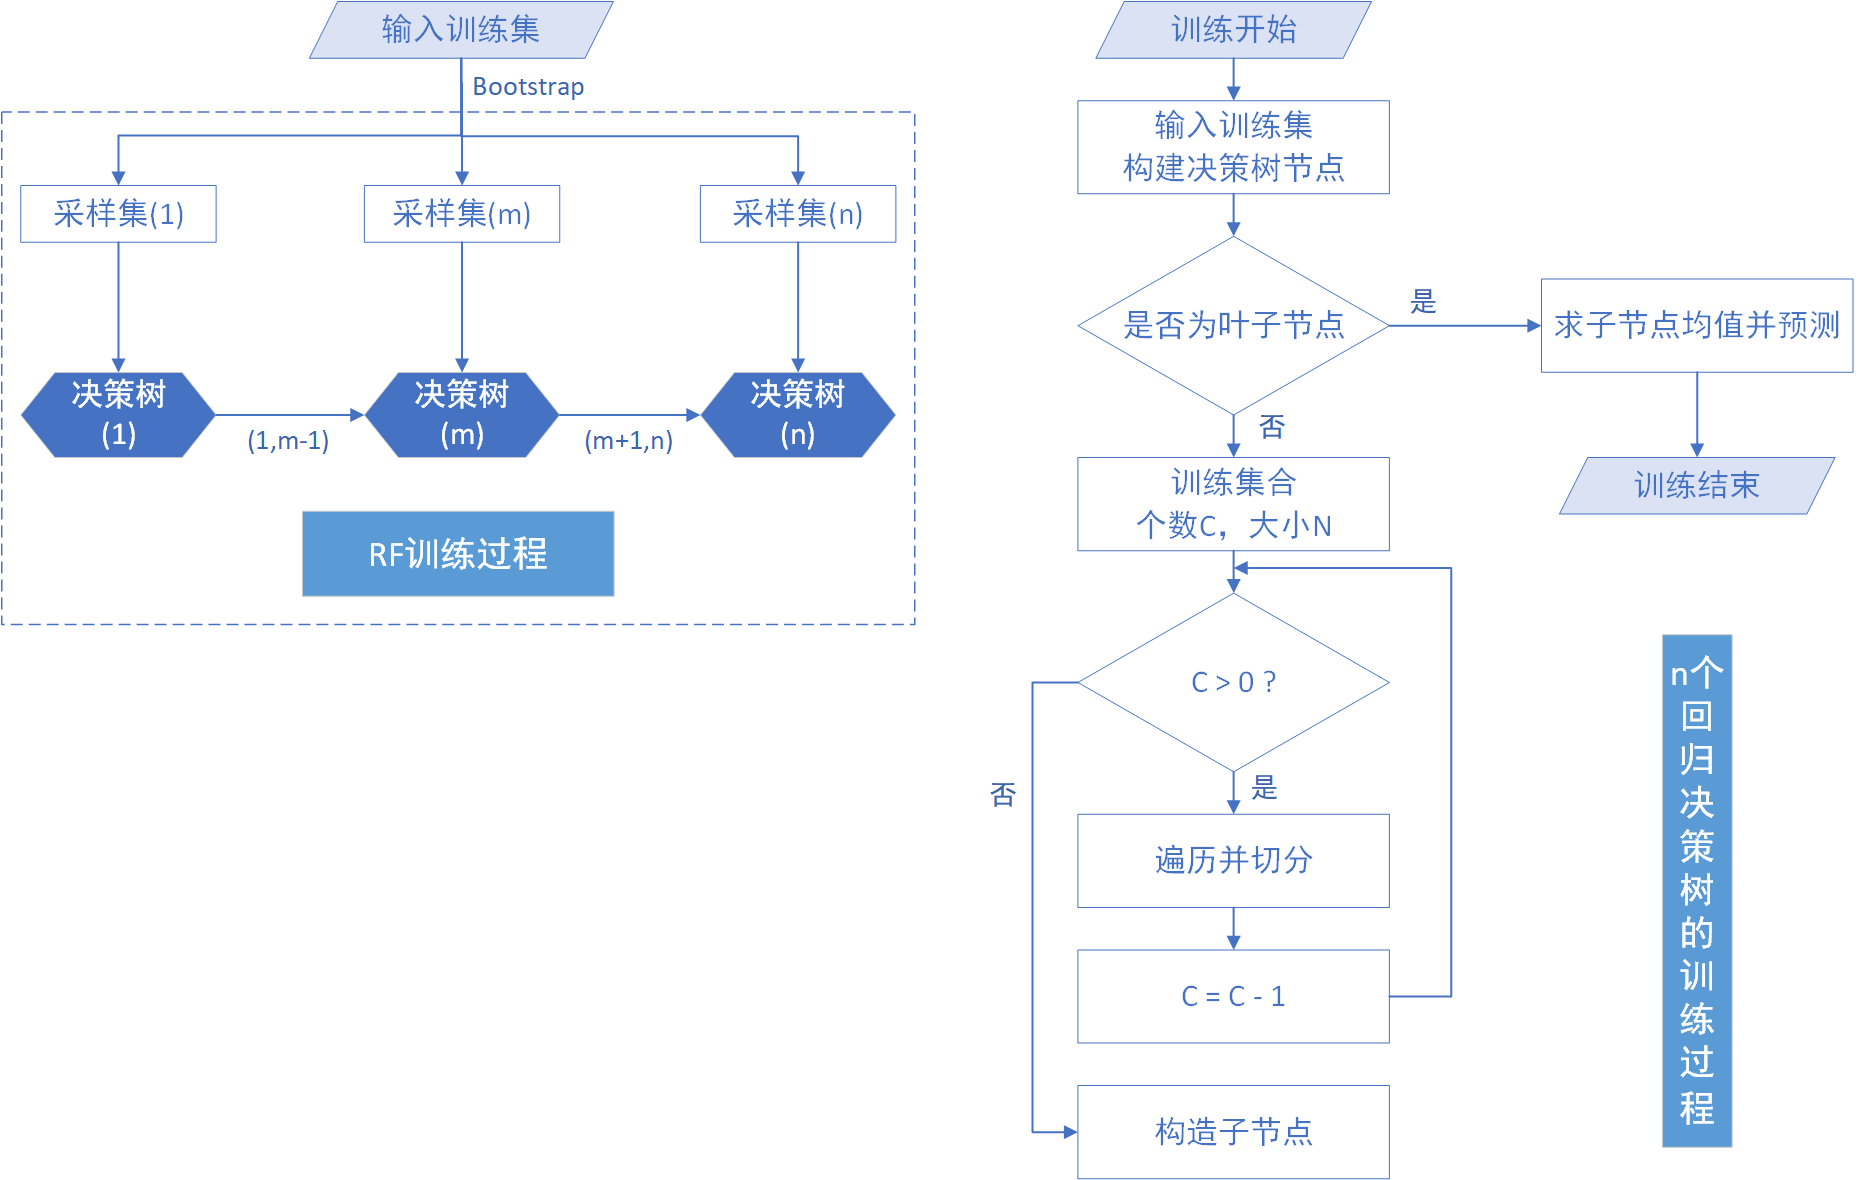
\includegraphics[width=\textwidth]{fig/RFflow.png}
	\caption{随机森林训练流程图}
	\label{fig:RFflow}
\end{figure}


随机森林的模型是将多个二叉决策树组合而成的,训练一个随机森林便是训练多个二叉决策树。在训练二叉决策树模型的时候需要考虑怎样选择分变量(特征) 、切分点以及怎样衡量一个切分变量、切分点的好坏。针对于切分变量和切分点的选择,采用穷举法,即遍历每个特征和每个特征的所有取值,最后从中找出最好的切分变量和切分点; 针对于切分变量和切分点的好坏, 一般以切分后节点的不纯度来衡量,即各个子节点不纯 度的加权和 $G\left(x_{i}, v_{i j}\right),$ 其计算公式如下
\begin{equation}
	G\left(x_{i}, v_{i j}\right)=\frac{n_{l e f t}}{N_{s}} H\left(\alpha_{l e f t}\right)+\frac{n_{r i g h t}}{N_{s}} H\left(\alpha_{r i g h t}\right)
\end{equation}

其中,$x_{i}$ 为某一个切分变量, $v_{i j}$ 为切分变量的一个切分值, $n_{l e f t}$、$n_{r i g h t}$、$N_{s}$ 分别为切分后左子节点的训练样本个数、右子节点的训练样本个数以及当前节点所有训练样本个数, $\alpha_{l e f t}$、$\alpha_{r i g h t}$ 分为左右子节点的训练样本集合, $H(X)$ 为衡量节点不纯度的函数。本模型中选用的是基尼不纯度 \cite{孙傲2019基于信息增益和基尼不纯度的},其定义如下:
\begin{equation}
H\left(\alpha_{m}\right)=\sum_{k} p_{m k} \left(1-p_{m k}\right)
\end{equation}
其中,$X_{m}$ 为当前节点的训练样本集合, $p_{m k}$ 为当前节点训练样本中 目标变量取值 $p_{m k}=\frac{N_{m k}}{N_{m}}$ 出现的概率。

决策树中某一节点的训练过程在数学上等价为即寻找 $G$ 最小的切分变量和切分点优化问题:
\begin{equation}
\left(x^{*}, v^{*}\right)=\operatorname{argmin}_{x, v} G\left(x_{i}, v_{i j}\right)
\end{equation}

计算特征重要性(Feature Importance),特征的重要性表示特征对预测结果影响程度,某一特征重要性越大,表明该特征对预测结果的影响越大,重要性越小,表明该特征对预测结果越小。某一节点 $k$ 的重要性为:
\begin{equation}
n_{k}=w_{k} * G_{k}-w_{l e f t} * G_{l e f t}-w_{r i g h t} * G_{r i g h t}
\end{equation}
其中, $w_{k}, w_{l e f t}, w_{r i g h t}$ 分别为节点 $k$ 以及其左右子节点中训练样本个数与总训练样本数目的 比例, $G_{k}, G_{l e f t}, G_{r i g h t}$ 分为为节点 $k$ 以及其左右子节点的不纯度。知道每一个节点的重要性之后, 即可通过公式(\ref{eq:fi})得出某一特征的重要性。
\begin{equation}\label{eq:fi}
f_{i}=\frac{\sum_{j \in n o d e s ~ s p l i t ~ o n ~ f e a t u r e ~i} n_j}{\sum_{k \in \text {all nodes}} n_{k}}
\end{equation}

为了使所有特征的重要性加起来等于1,需要每一特征的重要性进行归一化,公式如下:
\begin{equation}
f_{n i}=\frac{f_{i}}{\sum_{j \in \text {all features}} f_{j}}
\end{equation}

\subsubsection{信誉评级判定}
随机森林的预测判定结果是由内部所有二叉决策树的预测结果取平均值得到的。二叉决策树的预测判定过程主要分为以下步骤:
\begin{enumerate}
	\item 针对某一输入样本,从二叉决策树的根节点起,判断当前节点是否为叶子节点,如果是则返回叶子节点的预测值(即当前叶子中样本目标变量的平均值),如果不是则进入下一步;
	\item 根据当前节点的切分值进行移动;
	\item 循环步骤2,直到访问到叶子节点,并返回叶子节点的预测值。
\end{enumerate}

将预处理后的附件2中的企业指标带入训练后的模型进行信誉评级判定,得出了附件2中302所企业的信誉评级,其结果展示在附录\ref{ap:302}。



%%%%%%%%%%%%%%%%%%%%%%%%%%%%%%%%%%%%%%%%%%%%%%%%%%%%%%%%%%%%%%%%%%%%%%%%%%%
\section{问题三——基于朴素贝叶斯的文本分类}
\subsection{问题三的分析}
在企业的经营中,一些突发因素是不可避免的。例如2020年席卷全球的新冠疫情,让餐饮业、零售业、旅游业以及各种类型的个体企业受到了重大打击,然而对于一些医疗方面的企业反而可能会带来销售额上的大幅上涨。因此,企业的类别对企业应对不同类型的突发因素的表现不同,受其影响也不同。为了可以更加准确的估计企业的盈利额,进而评估企业的信贷风险,我们十分有必要将企业类型考虑到模型中去。
附件1和附件2中给出了企业的名称,但是数据量庞大,在短时间内使用人工分类的可能性很低,且不准确。因此我们使用自然语言处理(Natural Language Processing, NLP)的方法 \cite{陈肇雄1989自然语言处理,张钹2007自然语言处理的计算模型,李舟军2020面向自然语言处理的预训练技术研究综述},并结合朴素贝叶斯算法(Naive Bayes, NB) \cite{林江豪2012一种基于朴素贝叶斯的微博情感分类},对所给的公司名称进行分类 \cite{王垚尧0基于机器学习的经济行业分类方法研究},进而在问题一、二的模型基础上进行改进。



\subsection{自然语言处理}
将基于Python文本分析的生态化识别方法引入企业分类。首先进行数据清洗,使用Python完成对评论文本的NLP程序编写,可以有效分词去停、过滤附件中企业名称中的“*”号。分词主要运用Pynlpir模块中的Segment方法,此方法当前广泛应用于中文文本分析相关研究领域,具有较高的分词精准性 \cite{李筱瑜2019基于新词发现与词典信息的古籍文本分词研究,2019Study}。具体的自然语言处理步骤展示在 \ref{fig:NLP}。

\begin{figure}[h]
	\centering
	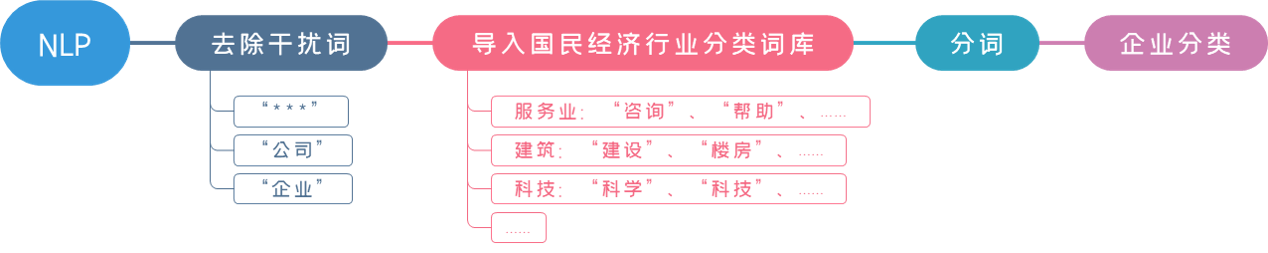
\includegraphics[width=\textwidth]{fig/NLP.png}
	\caption{自然语言处理步骤}
	\label{fig:NLP}
\end{figure}



\subsection{朴素贝叶斯文本分类}
以贝叶斯原理为基础的贝叶斯方法,运用了概率统计的知识对样本数据集进行分类。由于其具有着坚实的数学理论基础,贝叶斯分类算法的误判率是比较低的。朴素贝叶斯是一个非常简单,但是实用性很强的分类模型。朴素贝叶斯分类器的构造基础就是贝叶斯理论。

\subsubsection{贝叶斯公式}
贝叶斯公式的表示如下:
\begin{equation}\label{eq:NB}
	P(c_i \mid \beta)=\frac{P(\beta \mid C_i) P(c_i)}{P(\beta)}
\end{equation}
其中 $c_{i}$ 为类别, $\beta$ 为特征向量。

贝叶斯公式最常用于文本分类,公式(\ref{eq:NB})的左边可以理解为给定一个文本词向量$\beta$,那么它属于类别$c_i$的概率是多少。公式(\ref{eq:NB})的右边分三部分, $P(\beta \mid c_i)$ 表示了在给定类别的情况下,该文档的词向量的概率,其可以通过条件概率中的重要特性来求解。

\subsubsection{词袋法}
使用词袋法,且以《国民经济行业分类词库》 \cite{guominjingji} 训练集中的文本为词汇表,即将训练集中的文本中出现的单词(不重复)都统计出来作为词典,那么记单词的数目为$n$,这代表了文本的$n$个维度。

\subsubsection{TF计算方法}
使用词频 TF (Term Frequency) 的计算方法,为类别$y_k$每个词汇出现的次数 $N_{i}$,除以公司类别 $y_k$ 中词汇单词出现次数的总数 $N$:
\begin{equation}
P_{i}=\frac{N_{i}}{N}
\end{equation}

\subsubsection{拉普拉斯平滑}
为了避免训练集样本对一些特征的缺失,即某一些特征出现的次数为0,在计算 $P\left(X_{1}, X_{2}, X_{3}, \ldots, X_{n} \mid Y_{i}\right)$ 的时候,各个概率相乘最终结果为零,这样就会影响结果。我们对这个概率计算公式做了一个平滑处理:
\begin{equation}
P_{i}=\frac{N_{i}+\gamma}{N+\gamma * m}
\end{equation}
其中$m$为特征词向量的个数, $\gamma$为平滑系数, 当 $\gamma=1$时称为拉普拉斯平滑。


\subsection{模型求解}
使用《国民经济行业分类词库》 \cite{guominjingji} 进行训练分类后生成问题一中划分的12种企业类型,如图(\ref{fig:company})所示:餐饮业、城市建设、电器、服务业、工业、建筑与装饰、交通运输、科技密集型产业、零售业、农业、医疗、个体企业。

\begin{figure}[h]
	\centering
	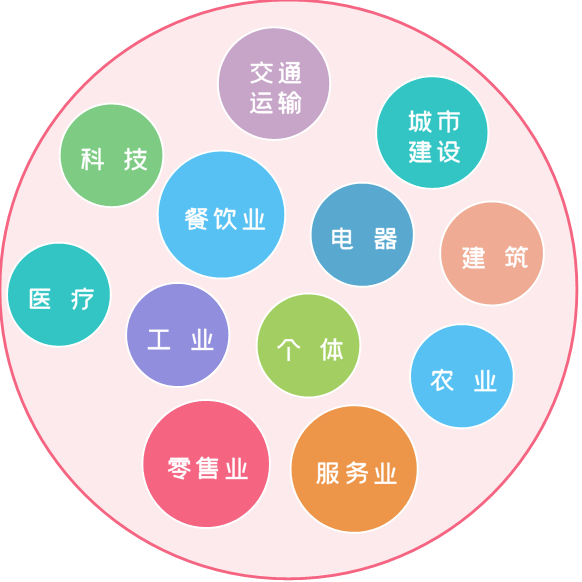
\includegraphics[width=0.4\textwidth]{fig/company}
	\caption{12种企业类型}
	\label{fig:company}
\end{figure}

将训练好的模型对附件1和附件2中的企业进行分类,得到的结果展示在图(\ref{fig:class}) 中。由于在问题一的数据预处理中,我们已经人工对123个公司进行了分类,将人工分类结果与模型分类结果相比较,符合率达到了93.47\%,说明分类效果很好,可信度较高。
\begin{figure}[h]
	\centering
	\includegraphics[width=\textwidth]{fig/class}
	\caption{企业分类结果}
	\label{fig:class}
\end{figure}

同一种突发因素对不同类型企业的影响程度不同,影响好坏也有区别。
例如一些医疗器械类型的企业,在疫情期间首批复工,发展迅速,Choice数据显示,截至8月19日,医药生物行业有157家上市公司发布2020年中报业绩预告,其中,超过72家企业业绩同向上升,但疫情期间的零售业、个体和交通运输业等等线下行业的利润严重下降,为了响应国家的号召,顾客疫情期间自我封闭管理,不出门不串门,对零售业和个体来说,这大大降低了其人流量,进而导致货品积压,资金链断裂;对交通运输业来说,客运单位均面临大量的线路取消、变更及旅客票务退改,对票务平台和客服部门带来极大的压力。
地震也是不可忽略的突发情况,地震后救治伤员所用的药品,尤其是疫苗和大输液,使医药行业大大受益,对提供衣食住行的农业与食品饮料行业也有良好的影响,但对于灾区的交通运输、供水供电、石油石化等公用事业公司,则产生偏负面的影响,进而影响到地震所在地的旅游景区。

图(\ref{fig:trend})为2019—2020年第一季度共五个季度的农业和零售业总产值柱形图,从图中我们可以看出,受疫情的影响,2020年第一季度农业、零售业总产值都大幅度下降,打破了持续增加的趋势。

\begin{figure}[h]
	\centering
	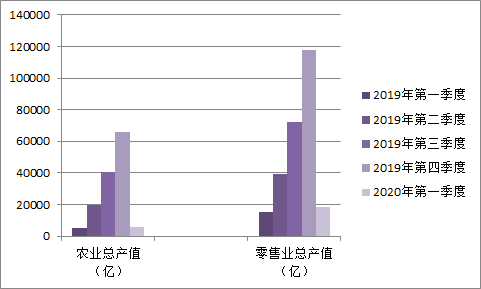
\includegraphics[width=0.7\textwidth]{fig/trend}
	\caption{2019—2020年第一季度共五个季度的农业和零售业总产值柱形图}
	\label{fig:trend}
\end{figure}


%%%%%%%%%%%%%%%%%%%%%%%%%%%%%%%%%%%%%%%%%%%%%%%%%%%%%%%%%%%%%%%%%%%%%%%%%%%
\section{模型的评价与推广}
\subsection{模型评价}
\subsubsection{模型优点}
\begin{itemize}
	\item 对附件中的数据进行了有效的数据清洗和数据预处理,使结果更加真实可靠,提高模型求解速度;
	\item 本文在正确、清晰地分析了题意的基础上,建立了合理、科学的企业信誉评级模型,为302家无信贷记录企业的分析提供了条件;
	\item 在假设的基础上建立了银行利润模型,巧妙地解决了不同信誉等级企业的不确定性;
	\item 建立的规划模型能与实际紧密联系,结合实际情况对问题进行求解,使得模型具有很好的通用性和推广性;
	\item 随机森林的算法能够有效地运行在大数据集上,且能够处理具有高维特征的输入样本,不需要降维。
	\item 计算采用专业的数学软件(MATLAB),可信度较高。
\end{itemize}

\subsubsection{模型缺点}
\begin{itemize}
	\item 本文将每个中小型企业都看作孤立个体,未考虑企业之间的相互影响,会与真实的结果产生偏差,也不能体现不同规模企业在授信额度上的差异;
	\item 本题是在理想的状态下求解的,现实的很多情况并没有考虑进去,中小型企业信贷的概率还可能受到国家经济形势与政策等多方面的影响;
	\item 由于只有企业的发票数据,缺失其他股份情况、负债情况、固定资产情况和与银行关系的信息,故只能根据企业的现金流数据对其违约风险进行分析量化;
	\item 授信额度侧重考虑银行收益最大化,对贷款额是否能满足企业的具体需求没有覆盖。
\end{itemize}

\subsection{模型推广}
本文通过一些理想化的假设,建立了银行利润模型和对中小型企业信誉评级的模型,适用领域广泛,实现了对数据属性不同、要求形式多样、限制条件多维情况下的分配方案的统筹分析,在提升资源利用率、节约生产成本、提高经济效益方面有着积极作用。


%参考文献
\newpage
\bibliographystyle{spbasic_unsort}
\bibliography{reference}
%\begin{thebibliography}{9}%宽度9
% \bibitem{bib:one} ....
% \bibitem{bib:two} ....
%\end{thebibliography}





%附录
\newpage
\begin{appendices}
\section{数据预处理以及指标生成--MATLAB源代码}
\begin{lstlisting}[language=MATLAB]
%% 进项发票总数和作废数量统计
type=cost{1,1};
sumType=0;
numType=1;
numNone=0;
for i = 1:210947               % 遍历所有数据
if cost{i,1}==type             % 如果还是这家企业
sumType=sumType+1;             % 企业的发票总数+1
if cost{i,4}=="作废发票"
numNone=numNone+1;
end
else
disp(type);                 % 监督进程
Rate{numType,5}=sumType;    % 将上一类的总数写入Rate文件
Rate{numType,6}=numNone;    % 将上一类的"作废发票"数量写入Rate文件
numType=numType+1;
type=cost{i,1};
sumType=1;
numNone=0;
end
if i==210947    % 特殊处理最后一类
disp(type);                 % 监督进程
Rate{numType,5}=sumType;    % 将上一类的总数写入Rate文件
Rate{numType,6}=numNone;    % 将上一类的"作废发票"数量写入Rate文件
end
end


%% 销项发票总数和作废数量统计
type=income{1,1};
sumType=0;
numType=1;
numNone=0;
for i = 1:162484               % 遍历所有数据
if income{i,1}==type           % 如果还是这家企业
sumType=sumType+1;             % 企业的发票总数+1
if income{i,4}=="作废发票"
numNone=numNone+1;
end
else
disp(type);                 % 监督进程
Rate{numType,7}=sumType;    % 将上一类的总数写入Rate文件
Rate{numType,8}=numNone;    % 将上一类的"作废发票"数量写入Rate文件
numType=numType+1;
type=income{i,1};
sumType=1;
numNone=0;
end
if i==162484    % 特殊处理最后一类
disp(type);                 % 监督进程
Rate{numType,7}=sumType;    % 将上一类的总数写入Rate文件
Rate{numType,8}=numNone;    % 将上一类的"作废发票"数量写入Rate文件
end
end


%% 年成本
resCostYear=zeros(123,5);     % 2016~2020
type=cost{1,1};               % 当前企业名称
numType=1;                    % 当前企业序数
t=strsplit(cost{1,2},"-");    % 分隔字符串
currentYear=t(1);             % 当前年
profitYear=0;                 % 本年利润

for i = 1:210947
% 时间转换
t=strsplit(cost{i,2},"-");
if cost{i,1}==type            % 如果还是这家企业
if t(1)==currentYear          % 进行年份累加
if cost{i,4}~="作废发票"       % 只计算有效发票
profitYear=profitYear-cost{i,3};
end
else                        % 如果到下一个年了
resCostYear(numType,str2double(t(1))-2015)=profitYear;    % 储存数据,存在第type行,第numYear列
disp(str2double(t(1))-1);
currentYear=t(1);         % 更新当前年
profitYear=0;             % 更新本年利润
if cost{i,4}~="作废发票"   % 只计算有效发票
profitYear=profitYear-cost{i,3};
end
end


else                       % 如果换了一个企业
disp(type);                % 监督进程
resCostYear(numType,str2double(t(1))-2015)=profitYear;    % 先把本企业的上一个年的数据储存
numType=numType+1;  % 更新企业序数
type=cost{i,1};           % 更新企业名称
currentYear=t(1);         % 更新当前年
profitYear=0;             % 更新本年利润
if cost{i,4}~="作废发票"   % 只计算有效发票
profitYear=profitYear-cost{i,3};
end
end

if i==210947    % 特殊处理最后一类
disp(type);                % 监督进程
resCostYear(numType,str2double(t(1))-2015)=profitYear;    % 先把上一个企业的最后一个月的数据储存
end
end


%% 年收入
resInYear=zeros(123,5);     % 2016~2020
type=income{1,1};           % 当前企业名称
numType=1;                  % 当前企业序数
t=strsplit(income{1,2},"-");    % 分隔字符串
currentYear=t(1);               % 当前年
profitYear=0;                   % 本年利润

for i = 1:162484
% 时间转换
t=strsplit(income{i,2},"-");
if income{i,1}==type             % 如果还是这家企业
if t(1)==currentYear             % 进行年份累加
if income{i,4}~="作废发票"        % 只计算有效发票
profitYear=profitYear+income{i,3};
end
else                        % 如果到下一个年了
resInYear(numType,str2double(t(1))-2015)=profitYear; % 储存数据,存在第numType行,第str2double(t(1))-2015列
disp(str2double(t(1))-1);  % 监督进程
currentYear=t(1);          % 更新当前年
profitYear=0;                     % 更新本年利润
if income{i,4}~="作废发票"         % 只计算有效发票
profitYear=profitYear+income{i,3};
end
end

else                            % 如果换了一个企业
disp(type);                     % 监督进程
resInYear(numType,str2double(t(1))-2015)=profitYear;    % 先把本企业的上一个年的数据储存
numType=numType+1;  % 更新企业序数
type=income{i,1};         % 更新企业名称
currentYear=t(1);         % 更新当前年
profitYear=0;             % 更新本年利润
if income{i,4}~="作废发票"         % 只计算有效发票
profitYear=profitYear+income{i,3};
end
end

if i==162484    % 特殊处理最后一类
disp(type);                     % 监督进程
resInYear(numType,str2double(t(1))-2015)=profitYear;    % 先把上一个企业的最后一个月的数据储存
end
end



%% 年利润
resProfit=resInYear+resCostYear;

%% 进项负数发票数量
type=cost{1,1};
numType=1;
numNone=0;
for i = 1:210947           % 遍历所有数据
if cost{i,1}==type         % 如果还是这家企业
if cost{i,3}<0
numNone=numNone+1;
end
else
disp(type);                 % 监督进程
Rate{numType,5}=numNone;    % 将上一类的"作废发票"数量写入Rate文件
numType=numType+1;
type=cost{i,1};
numNone=0;
end
if i==210947    % 特殊处理最后一类
disp(type);                 % 监督进程
Rate{numType,5}=numNone;    % 将上一类的"作废发票"数量写入Rate文件
end
end


%% 销项负数发票数量
type=income{1,1};
numType=1;
numNone=0;
for i = 1:162484              % 遍历所有数据
if income{i,1}==type          % 如果还是这家企业
if income{i,3}<0
numNone=numNone+1;
end
else
disp(type);                 % 监督进程
Rate{numType,5}=numNone;    % 将上一类的"作废发票"数量写入Rate文件
numType=numType+1;
type=income{i,1};
numNone=0;
end
if i==162484    % 特殊处理最后一类
disp(type);                 % 监督进程
Rate{numType,5}=numNone;    % 将上一类的"作废发票"数量写入Rate文件
end
end


%% 违约率的三个参数
resBreak=zeros(4,3);
RankArr=["A" "B" "C" "D"];
for rank=1:4
sumBreak=0;
sumRankType=0;
sumObs=0;
sumNeg=0;
for i = 1:123
if Break{i,4}==RankArr(rank)
sumRankType=sumRankType+1;
sumObs=sumObs+Break{i,6}+Break{i,7};
sumNeg=sumNeg+Break{i,8}+Break{i,9};
if Break{i,5}==1
sumBreak=sumBreak+1;
end
end
end
resBreak(rank,1)=sumBreak/sumRankType;
resBreak(rank,2)=sumObs/sumRankType/2;
resBreak(rank,3)=sumNeg/sumRankType/2;
end


%% 年均利润
res=zeros(123,1);
for i=1:123
p=0;
num=0;
if Total{i,16}~=0
p=p+Total{i,16};
num=num+1;
end
if Total{i,17}~=0
p=p+Total{i,17};
num=num+1;
end
if Total{i,18}~=0
p=p+Total{i,18};
num=num+1;
end
if Total{i,19}~=0
p=p+Total{i,19};
num=num+1;
end
if Total{i,20}~=0
p=p+Total{i,20};
num=num+1;
end
res(i,1)=p/num;
end
\end{lstlisting}
	
\section{随机森林进行信誉等级评定--Python源代码}
\begin{lstlisting}[language=Python]
from sklearn.model_selection import train_test_split, GridSearchCV
from sklearn.feature_extraction import DictVectorizer
from sklearn.externals import joblib
from sklearn.ensemble import RandomForestClassifier
import pandas as pd


def decision():
"""
随机森林进行信誉等级评定
:return: acc--模型准确率
"""
# 获取数据
data_orig = pd.read_csv("data.csv")
# 处理数据,找出特征值和目标值
x = data_orig[['是否违约(0-否,1-是)', '进项作废比', '销项作废比', '进项负数比', '销项负数比', '年均利润']]
y = data_orig['信誉评级']
# 分割数据集到训练集合测试集
x_train, x_test, y_train, y_test = train_test_split(x, y, test_size=0.25)
# 进行处理(特征工程)特征->类别->one_hot编码
dic = DictVectorizer(sparse=False)
x_train = dic.fit_transform(x_train.to_dict(orient="records"))
print(dic.get_feature_names())
x_test = dic.transform(x_test.to_dict(orient="records"))
# 随机森林进行预测 (超参数调优)
rf = RandomForestClassifier(n_jobs=-1)
param = {"n_estimators": [50, 120, 200, 300], "max_depth": [5, 8, 15, 25, 30, 50]}
# 网格搜索与交叉验证
gc = GridSearchCV(rf, param_grid=param, cv=2)
gc.fit(x_train, y_train)
acc = gc.score(x_test, y_test)
print("准确率:", acc)
print("查看选择的参数模型:", gc.best_params_)
joblib.dump(gc, 'rf.pkl')
return acc


if __name__ == "__main__":
while 1:
accuracy = decision()
if accuracy > 0.7:
break

# 获取数据
data = pd.read_csv("dataTest.csv")
# 处理数据,找出特征值
x = data[['是否违约(0-否,1-是)', '进项作废比', '销项作废比', '进项负数比', '销项负数比', '年均利润']]
# 加载模型
new_rf = joblib.load('rf.pkl')
print(new_rf.predict(x))
\end{lstlisting}


\section{朴素贝叶斯进行文本分类--Python源代码}
\begin{lstlisting}[language=Python]
from sklearn.datasets import fetch_20newsgroups
from sklearn.model_selection import train_test_split
from sklearn.feature_extraction.text import TfidfVectorizer
from sklearn.naive_bayes import MultinomialNB
from sklearn.metrics import classification_report

def naviebayes():
"""
朴素贝叶斯进行文本分类
:return: None
"""
news = fetch_20newsgroups(subset='all')
# 进行数据分割
x_train, x_test, y_train, y_test = train_test_split(news.data, news.target, test_size=0.25)
# 对数据集进行特征抽取
tf = TfidfVectorizer()
# 以训练集当中的词的列表进行每个词的重要性统计
x_train = tf.fit_transform(x_train)
print(tf.get_feature_names())
x_test = tf.transform(x_test)
# 进行朴素贝叶斯算法的预测
mlt = MultinomialNB(alpha=1.0)
print(x_train.toarray())
mlt.fit(x_train, y_train)
y_predict = mlt.predict(x_test)
print("预测的公司类别为:", y_predict)
# 得出准确率
print("准确率为:", mlt.score(x_test, y_test))
print("每个类别的精确率和召回率:", classification_report(y_test, y_predict, target_names=news.target_names))
return None

if __name__ == "__main__":
naviebayes()
\end{lstlisting}
 

\newpage
\section{问题二中302家企业信誉评级结果} \label{ap:302}
\begin{table}[h]
	\begin{center}
		\begin{tabular}{|c|c|c|c|c|c|c|c|c|c|}
			\hline
			E124 & E125 & E126 & E127 & E128 & E129 & E130 & E131 & E132 & E133 \\ 
			B & B & B & C & B & B & C & B & B & B \\ \hline
			E134 & E135 & E136 & E137 & E138 & E139 & E140 & E141 & E142 & E143 \\ 
			B & B & C & B & A & C & B & C & B & A \\ \hline
			E144 & E145 & E146 & E147 & E148 & E149 & E150 & E151 & E152 & E153 \\ 
			B & B & B & A & C & C & B & C & A & C \\ \hline
			E154 & E155 & E156 & E157 & E158 & E159 & E160 & E161 & E162 & E163 \\ 
			A & A & B & B & B & B & B & C & B & B \\ \hline
			E164 & E165 & E166 & E167 & E168 & E169 & E170 & E171 & E172 & E173 \\ 
			B & B & B & B & C & C & C & B & B & A \\ \hline
			E174 & E175 & E176 & E177 & E178 & E179 & E180 & E181 & E182 & E183 \\ 
			B & B & B & B & B & B & A & B & C & B \\ \hline
			E184 & E185 & E186 & E187 & E188 & E189 & E190 & E191 & E192 & E193 \\ 
			C & A & A & B & C & C & B & A & B & B \\ \hline
			E194 & E195 & E196 & E197 & E198 & E199 & E200 & E201 & E202 & E203 \\ 
			C & A & B & C & B & C & B & B & C & B \\ \hline
			E204 & E205 & E206 & E207 & E208 & E209 & E210 & E211 & E212 & E213 \\ 
			B & A & C & C & B & B & B & B & C & B \\ \hline
			E214 & E215 & E216 & E217 & E218 & E219 & E220 & E221 & E222 & E223 \\ 
			B & C & B & B & B & B & A & C & B & B \\ \hline
			E224 & E225 & E226 & E227 & E228 & E229 & E230 & E231 & E232 & E233 \\ 
			C & B & B & B & B & B & B & B & A & C \\ \hline
		\end{tabular}
	\end{center}
\end{table}
\begin{table}[h]
	\begin{center}
		\begin{tabular}{|c|c|c|c|c|c|c|c|c|c|}
			\hline
			E234 & E235 & E236 & E237 & E238 & E239 & E240 & E241 & E242 & E243 \\ 
			C & C & B & B & B & B & B & B & B & C \\ \hline
			E244 & E245 & E246 & E247 & E248 & E249 & E250 & E251 & E252 & E253 \\ 
			B & B & B & B & B & C & B & B & C & B \\ \hline
			E254 & E255 & E256 & E257 & E258 & E259 & E260 & E261 & E262 & E263 \\ 
			C & B & A & B & A & B & B & B & C & B \\ \hline
			E264 & E265 & E266 & E267 & E268 & E269 & E270 & E271 & E272 & E273 \\ 
			B & B & B & C & C & B & B & B & B & C \\ \hline
			E274 & E275 & E276 & E277 & E278 & E279 & E280 & E281 & E282 & E283 \\ 
			C & B & B & C & B & C & C & C & B & C \\ \hline
			E284 & E285 & E286 & E287 & E288 & E289 & E290 & E291 & E292 & E293 \\ 
			B & B & C & B & B & B & B & B & C & C \\ \hline
			E294 & E295 & E296 & E297 & E298 & E299 & E300 & E301 & E302 & E303 \\ 
			B & B & B & C & B & B & B & B & B & B \\ \hline
			E304 & E305 & E306 & E307 & E308 & E309 & E310 & E311 & E312 & E313 \\ 
			B & C & B & C & B & B & B & B & A & B \\ \hline
			E314 & E315 & E316 & E317 & E318 & E319 & E320 & E321 & E322 & E323 \\ 
			B & A & B & B & B & B & C & B & A & B \\ \hline
			E324 & E325 & E326 & E327 & E328 & E329 & E330 & E331 & E332 & E333 \\ 
			B & A & C & C & B & C & C & B & C & B \\ \hline
			E334 & E335 & E336 & E337 & E338 & E339 & E340 & E341 & E342 & E343 \\ 
			C & C & C & C & B & C & B & C & B & C \\ \hline
		\end{tabular}
	\end{center}
\end{table}

\begin{table}[h]
	\begin{center}
		\begin{tabular}{|c|c|c|c|c|c|c|c|c|c|}
			\hline
			E344 & E345 & E346 & E347 & E348 & E349 & E350 & E351 & E352 & E353 \\ 
			A & C & B & C & A & C & B & B & B & B \\ \hline
			E354 & E355 & E356 & E357 & E358 & E359 & E360 & E361 & E362 & E363 \\ 
			C & C & C & A & B & C & C & C & B & B \\ \hline
			E364 & E365 & E366 & E367 & E368 & E369 & E370 & E371 & E372 & E373 \\ 
			B & B & C & B & B & C & C & C & B & C \\ \hline
			E374 & E375 & E376 & E377 & E378 & E379 & E380 & E381 & E382 & E383 \\ 
			C & C & C & C & B & B & B & B & C & B \\ \hline
			E384 & E385 & E386 & E387 & E388 & E389 & E390 & E391 & E392 & E393 \\ 
			C & C & C & C & C & B & B & B & C & C \\ \hline
			E394 & E395 & E396 & E397 & E398 & E399 & E400 & E401 & E402 & E403 \\ 
			B & B & B & C & C & C & C & C & B & C \\ \hline
			E404 & E405 & E406 & E407 & E408 & E409 & E410 & E411 & E412 & E413 \\ 
			B & C & B & B & C & C & A & B & C & C \\ \hline
			E414 & E415 & E416 & E417 & E418 & E419 & E420 & E421 & E422 & E423 \\ 
			C & C & C & C & C & C & B & C & C & B \\ \hline
			E424 & E425 & & & & & & & & \\ 
			B & B & & & & & & & & \\ \hline
		\end{tabular}
	\end{center}
	%}
\end{table}

 
\end{appendices}

\end{document} 